% Preamble
\documentclass[xcolor=table,handout]{beamer}

% Title/Author/Date
\title{Introduction to Robotframework}  
\author[K. Bellock]{Kenneth Bellock}
\titlegraphic{%
    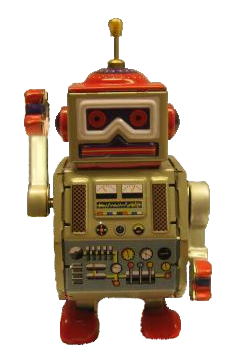
\includegraphics[height=.37\textheight]{robot-wave}

    \tiny \url{http://robotframework.org}
}
\date{\vspace*{-2.5em}\par \today} 

% Package Dependencies
\usepackage{beamerthemeshadow}
\usepackage{color}
\usepackage{colortbl}
\usepackage{booktabs}
\usepackage{adjustbox}
\usepackage{lmodern}
\usepackage{tikz}
\usepackage{pgfpages}
\usepackage{pgfgantt}
\usepackage{pgfcalendar}
\usepackage{pgfplots}
\pgfplotsset{compat=newest}
\usepackage{calc}
\usepackage{ifthen}
\usepackage{tcolorbox}
\usepackage[edges]{forest}
\tcbuselibrary{theorems,listings,skins,breakable,minted}
\usetikzlibrary{shapes, arrows, intersections}
\setbeamercolor{bgcolor}{fg=black,bg=blue!10}
\definecolor{foldercolor}{RGB}{124,166,198}
\usepackage[printwatermark]{xwatermark}

% Draft Watermark
\definecolor{draftcolor}{rgb}{0.7, 0.8, 0.1}
\newsavebox\mybox{}
\savebox\mybox{\tikz[opacity=0.35]\node{\textcolor{draftcolor}{DRAFT}};}
\newwatermark*[
  allpages,
  angle=45,
  scale=8,
  xpos=-25,
  ypos=25]{\usebox\mybox}

% Handouts
% \pgfpagesuselayout{2 on 1}[letterpaper,border shrink=5mm]
% \pgfpageslogicalpageoptions{1}{border code=\pgfusepath{stroke}}
% \pgfpageslogicalpageoptions{2}{border code=\pgfusepath{stroke}}
% \pgfpageslogicalpageoptions{3}{border code=\pgfusepath{stroke}}
% \pgfpageslogicalpageoptions{4}{border code=\pgfusepath{stroke}}
% \setbeameroption{show notes}

%  Presentation with Notes
% \setbeameroption{show notes}
% \setbeameroption{show notes on second screen=right}

%  Notes
% \setbeameroption{show only notes}

% Disable Navigation Symbols
\setbeamertemplate{navigation symbols}{}

% Set Caption Options
\setbeamertemplate{caption}[numbered]
\setbeamerfont{caption}{size=\tiny}

% Directory Tree Settings
\tikzset{pics/folder/.style={code={%
    \node[inner sep=0pt, minimum size=#1](-foldericon){};
    \node[folder style, inner sep=0pt, minimum width=0.3*#1, minimum height=0.6*#1, above right, xshift=0.05*#1] at (-foldericon.west){};
    \node[folder style, inner sep=0pt, minimum size=#1] at (-foldericon.center){};}
    },
    pics/folder/.default={20pt},
    folder style/.style={draw=foldercolor!80!black,top color=foldercolor!40,bottom color=foldercolor}
}
\forestset{is file/.style={edge path'/.expanded={%
        ([xshift=\forestregister{folder indent}]!u.parent anchor) |- (.child anchor)},
        inner sep=1pt},
    this folder size/.style={edge path'/.expanded={%
        ([xshift=\forestregister{folder indent}]!u.parent anchor) |- (.child anchor) pic[solid]{folder=#1}}, inner ysep=0.6*#1},
    folder tree indent/.style={before computing xy={l=#1}},
    folder icons/.style={folder, this folder size=#1, folder tree indent=3*#1},
    folder icons/.default={12pt},
}

% New counter for Listings
\newcounter{listings}

\begin{document}

\section{Introduction}

\begin{frame}% Title Frame
  \titlepage{}
  \note{Assumptions:}
  \note[item]{TODO:\@ List assumptions.}
\end{frame}

\begin{frame}\frametitle{Table of contents}
  \tableofcontents{}
  \note[item]{A road map is a great thing to have.}
  \note[item]{A joke or reference to current events in common culture would be great here if the audience appears receptive.}
\end{frame} 

\begin{frame}\frametitle{Objectives}
    %TODO: List folder structure and buildup of RF principles into increasingly more feature rich examples, included in objectives is the goal that all that should be needed is a python installation, virtualenv, and this guide to complete all the actions in this training
    % Include discussion of how there is no "Right Way" think "Way of the Robot", what I layout here is my own method of organizing robotframework components
\end{frame}

\begin{frame}\frametitle{Directory Organization}
    \begin{columns}
        \begin{column}[T]{0.50\textwidth}
            \begin{itemize}\footnotesize
                \item There is no \emph{``Way of the Robot''} when it comes to organizing your project
                \item The framework is designed to be flexible, so you can define any organization you want, but this causes a lot of trouble for beginners and often results in projects where everything is just dumped into one big pot
                \item For these examples, we will use the Filesystem Hierarchy Standard (\url{https://en.wikipedia.org/wiki/Filesystem_Hierarchy_Standard}
            \end{itemize}
        \end{column}
        \begin{column}[T]{0.50\textwidth}
    \begin{adjustbox}{width=\textwidth}
    \begin{forest}
    for tree={font=\sffamily, %grow'=0,
    folder indent=.9em, folder icons,
    edge=densely dotted}
    [test
      % [images, this folder size=20pt
      %     [wallpapers]
      %     [logo.pdf, is file]]
      [etc, this folder size=20pt]
      [lib, this folder size=20pt]
      [src, this folder size=20pt]
      [var, this folder size=20pt]
      [tmp, this folder size=20pt]
    ]
  \end{forest}
\end{adjustbox}
            \begin{description}
                \item[etc] Resource Files
                \item[lib] Libraries
                \item[src] Test Suites
                \item[var] Variables
                \item[tmp] Temporary Files
            \end{description}
\end{column}
\end{columns}
\end{frame}

\begin{frame}\frametitle{What is Robotframework?}
\vfill
\textbf{From their webpage:}
\vfill
    \emph{Robot Framework is a generic test automation framework for acceptance testing and acceptance test-driven development (ATDD). It has easy-to-use tabular test data syntax and it utilizes the keyword-driven testing approach. Its testing capabilities can be extended by test libraries implemented either with Python or Java, and users can create new higher-level keywords from existing ones using the same syntax that is used for creating test cases.}
\vfill
\end{frame}

\section{Installation}

\begin{frame}[fragile]\frametitle{Installation}

    \begin{itemize}
        \item Virtualenv (\url{https://virualenv.pypa.io}), is a tool to create isolated Python environments; as demonstrated in Listing~\ref{lst:virtualenv}, it will provide the capability to install python toolboxes without administrator priveledges
        \item For these examples, I will use the locally qualified path to a virtual environment we are going to create
        \item If you already have an installation of robotframework available, substitute the path to your installation
    \end{itemize}
\vfill
\begin{tcblisting}{%
     theorem={Listing}{listings}{Install Robotframework}{lst:virtualenv},
     fonttitle=\scriptsize\bfseries,
     listing engine=minted,
     minted language=shell-session,
     minted options={%
         breaklines,
         fontsize=\tiny,
         numbersep=2mm,
         baselinestretch=1,
         linenos},
     overlay={%
       \begin{tcbclipinterior}
           \fill[gray!25] (frame.south west) rectangle ([xshift=4mm]frame.north west);
       \end{tcbclipinterior}},
     breakable, enhanced, listing only}
>> virtualenv local
>> local/bin/pip install robotframework
\end{tcblisting}
\end{frame}

\end{document}
